The matching consist on link objects between both images. It's an essential step in the algorithm because without step is not possible to track rightly 3D targets.\\

\begin{figure} [h]
	\centering
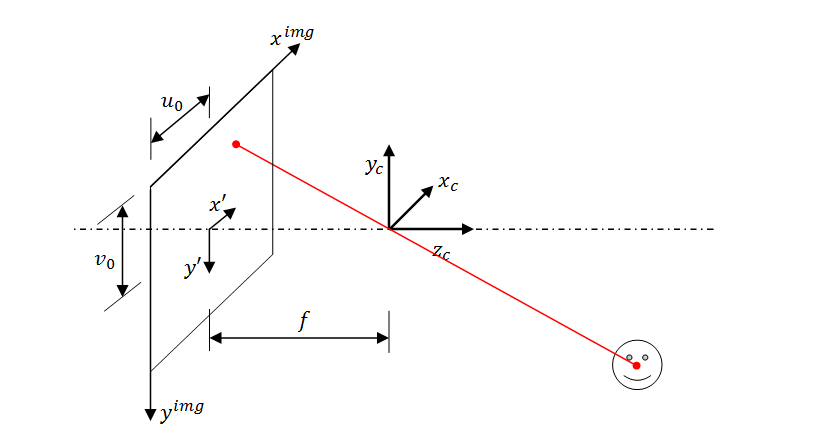
\includegraphics[width=0.75\textwidth,natwidth=544,natheight=388]{../Images/c1/pinhole_model.png} 
	\caption{Pinhole Camera Model}
	\label{fig:Pinhole_Model}
\end{figure}

Firstly, in this article it's assumed that camera's behavior is governed by the pinhole model. According to this and assuming that the X axis of the camera define its the orientation, every space point (X,Y,Z) has the following projection. \\

\begin{equation} \label{eq:pinhole_cam_eq}
\begin{split}
X^{img} = f*\frac{Y}{X} \\
Y^{img} = f*\frac{Z}{X}
\end{split}
\end{equation}

Where f is the focal length of the camera; $X^{img}$ and $Y^{img}$ are the projection of the three dimensional point on the camera plane. This equations are in $\mathbb{R}^3$ the equations of 2 planes that cut in one line (The epipolar line). So in conclusion, every segmented object in the camera's images provide a pair of planes (or a single line). Ideally, if the Segmentation had no errors every pair os lines (One per camera for the same target) will cross in a point. However due to errors is almost improbable. That's why the matching algorithm links the objects by minimizing the distance between lines.

\begin{figure}[h]
\centering
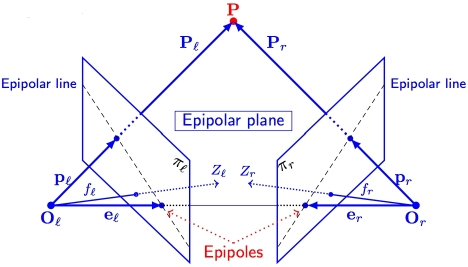
\includegraphics[width=0.75\textwidth,natwidth=468,natheight=267]{../Images/c1/Epipolar_Lines.png}
\caption{Epipolar Lines}
\label{fig:Epipolar_Lines}
\end{figure}

To be precise, the obtained image in the computer hasn't got negative projection. The values on the image are displaced vertically and horizontally. This displacement is stored as the camera�s image centroid or $(u_0, v_0)$. Eventually, equations are: \\

\begin{align}
X^{img} = f*\frac{Y}{X} + u_0 \\
Y^{img} = f*\frac{Z}{X} + v_0
\end{align}


Due to the noise in the pictures and in the positioning sensors, the pairs of lines would not ever cut. So that, the application minimize the distance between those lines ( \ref{fig:line-min-dist} ). \\
Let be $P_1$ and $P_2$ two points (The first one belong to the line $r_1$ and the second one to $r_2$). This point are defined respectively as: \\

\begin{align}
P_1 = P_1^0 + u_1 * s \\
P_2 = P_2^0 + u_2 * t
\end{align}


Given the definition of these points, the segment $\overline{P_1P_2}$ will be: \\

\begin{equation}
\overline{P_1P_2}=(P_2^0 - P_1^0) + (u_2 * t - u_1 * s)
\end{equation}


The minimal distance is defined as the length of the segment perpendicular to both lines. Mathematically, $\overline{P_1P_2} * u1 = 0$ and $\overline{P_1P_2} * u2 = 0$. Operating with both equations:

\begin{align}
s = \frac{\frac{u_2 * u_2}{u_2 * u_1}*(P_2 - P_1) * u_1 - (P_2 - P_1) * u_2}{\frac{u_2 * u_2}{u_2 * u_1}(u_1 * u_1) - u_1*u_2}	\\
t = \frac{u_1 *_u1 * s - [P_2 - P_1] * u_1}{u_2 * u_1}
\end{align}

Eventually, $dist(r_1,r_2) = norm(\overline{P_1P_2(s,t)})$.

\begin{figure}[h]
\centering
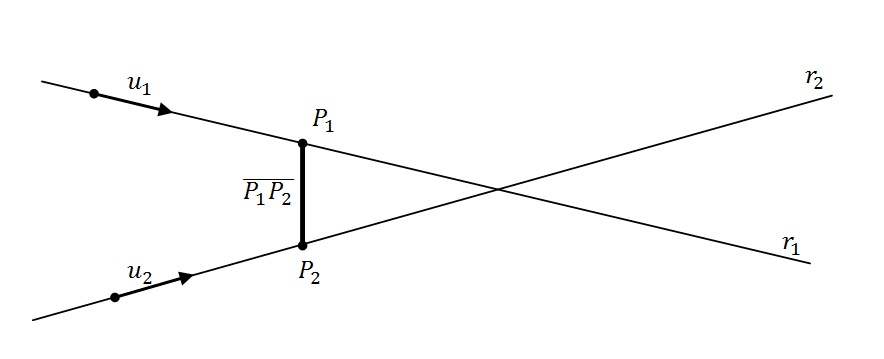
\includegraphics[width=0.7\linewidth]{../Images/c1/line_cut}
\caption{Line minimal distance}
\label{fig:line-min-dist}
\end{figure}


